% Template for PLoS
% Version 3.5 March 2018
%
% % % % % % % % % % % % % % % % % % % % % %
%
% -- IMPORTANT NOTE
%
% This template contains comments intended 
% to minimize problems and delays during our production 
% process. Please follow the template instructions
% whenever possible.
%
% % % % % % % % % % % % % % % % % % % % % % % 
%
% Once your paper is accepted for publication, 
% PLEASE REMOVE ALL TRACKED CHANGES in this file 
% and leave only the final text of your manuscript. 
% PLOS recommends the use of latexdiff to track changes during review, as this will help to maintain a clean tex file.
% Visit https://www.ctan.org/pkg/latexdiff?lang=en for info or contact us at latex@plos.org.
%
%
% There are no restrictions on package use within the LaTeX files except that 
% no packages listed in the template may be deleted.
%
% Please do not include colors or graphics in the text.
%https://www.overleaf.com/project/5c531f8b9a96997f58470c6f
% The manuscript LaTeX source should be contained within a single file (do not use \input, \externaldocument, or similar commands).
%
% % % % % % % % % % % % % % % % % % % % % % %
%
% -- FIGURES AND TABLES
%
% Please include tables/figure captions directly after the paragraph where they are first cited in the text.
%
% DO NOT INCLUDE GRAPHICS IN YOUR MANUSCRIPT
% - Figures should be uploaded separately from your manuscript file. 
% - Figures generated using LaTeX should be extracted and removed from the PDF before submission. 
% - Figures containing multiple panels/subfigures must be combined into one image file before submission.
% For figure citations, please use "Fig" instead of "Figure".
% See http://journals.plos.org/plosone/s/figures for PLOS figure guidelines.
%
% Tables should be cell-based and may not contain:
% - spacing/line breaks within cells to alter layout or alignment
% - do not nest tabular environments (no tabular environments within tabular environments)
% - no graphics or colored text (cell background color/shading OK)
% See http://journals.plos.org/plosone/s/tables for table guidelines.
%
% For tables that exceed the width of the text column, use the adjustwidth environment as illustrated in the example table in text below.
%
% % % % % % % % % % % % % % % % % % % % % % % %
%
% -- EQUATIONS, MATH SYMBOLS, SUBSCRIPTS, AND SUPERSCRIPTS
%
% IMPORTANT
% Below are a few tips to help format your equations and other special characters according to our specifications. For more tips to help reduce the possibility of formatting errors during conversion, please see our LaTeX guidelines at http://journals.plos.org/plosone/s/latex
%
% For inline equations, please be sure to include all portions of an equation in the math environment.  For example, x$^2$ is incorrect; this should be formatted as $x^2$ (or $\mathrm{x}^2$ if the romanized font is desired).
%
% Do not include text that is not math in the math environment. For example, CO2 should be written as CO\textsubscript{2} instead of CO$_2$.
%
% Please add line breaks to long display equations when possible in order to fit size of the column. 
%
% For inline equations, please do not include punctuation (commas, etc) within the math environment unless this is part of the equation.
%
% When adding superscript or subscripts outside of brackets/braces, please group using {}.  For example, change "[U(D,E,\gamma)]^2" to "{[U(D,E,\gamma)]}^2". 
%
% Do not use \cal for caligraphic font.  Instead, use \mathcal{}
%
% % % % % % % % % % % % % % % % % % % % % % % % 
%
% Please contact latex@plos.org with any questions.
%
% % % % % % % % % % % % % % % % % % % % % % % %

\documentclass[10pt,letterpaper]{article}
\usepackage[top=0.85in,left=2.75in,footskip=0.75in]{geometry}

% amsmath and amssymb packages, useful for mathematical formulas and symbols
\usepackage{amsmath,amssymb}

% Use adjustwidth environment to exceed column width (see example table in text)
\usepackage{changepage}

% Use Unicode characters when possible
\usepackage[utf8x]{inputenc}

% textcomp package and marvosym package for additional characters
\usepackage{textcomp,marvosym}

% cite package, to clean up citations in the main text. Do not remove.
\usepackage{cite}

% Use nameref to cite supporting information files (see Supporting Information section for more info)
\usepackage{nameref,hyperref}

% line numbers
%\usepackage[right]{lineno}

% ligatures disabled
\usepackage{microtype}
\DisableLigatures[f]{encoding = *, family = * }

% color can be used to apply background shading to table cells only
\usepackage[table]{xcolor}

% array package and thick rules for tables
\usepackage{array}

% create "+" rule type for thick vertical lines
\newcolumntype{+}{!{\vrule width 2pt}}

% create \thickcline for thick horizontal lines of variable length
\newlength\savedwidth
\newcommand\thickcline[1]{%
  \noalign{\global\savedwidth\arrayrulewidth\global\arrayrulewidth 2pt}%
  \cline{#1}%
  \noalign{\vskip\arrayrulewidth}%
  \noalign{\global\arrayrulewidth\savedwidth}%
}

% \thickhline command for thick horizontal lines that span the table
\newcommand\thickhline{\noalign{\global\savedwidth\arrayrulewidth\global\arrayrulewidth 2pt}%
\hline
\noalign{\global\arrayrulewidth\savedwidth}}


% Remove comment for double spacing
%\usepackage{setspace} 
%\doublespacing

% Text layout
\raggedright
\setlength{\parindent}{0.5cm}
\textwidth 5.25in 
\textheight 8.75in

% Bold the 'Figure #' in the caption and separate it from the title/caption with a period
% Captions will be left justified
\usepackage[aboveskip=1pt,labelfont=bf,labelsep=period,justification=raggedright,singlelinecheck=off]{caption}
\renewcommand{\figurename}{Fig}

% Use the PLoS provided BiBTeX style
\bibliographystyle{plos2015}

% Remove brackets from numbering in List of References
\makeatletter
\renewcommand{\@biblabel}[1]{\quad#1.}
\makeatother



% Header and Footer with logo
\usepackage{lastpage,fancyhdr,graphicx}
\usepackage{epstopdf}
%\pagestyle{myheadings}
\pagestyle{fancy}
\fancyhf{}
%\setlength{\headheight}{27.023pt}
%\lhead{\includegraphics[width=2.0in]{PLOS-submission.eps}}
\rfoot{\thepage/\pageref{LastPage}}
\renewcommand{\headrulewidth}{0pt}
\renewcommand{\footrule}{\hrule height 2pt \vspace{2mm}}
\fancyheadoffset[L]{2.25in}
\fancyfootoffset[L]{2.25in}
\lfoot{\today}

%% Include all macros below

\newcommand{\lorem}{{\bf LOREM}}
\newcommand{\ipsum}{{\bf IPSUM}}

%% END MACROS SECTION


\begin{document}
\vspace*{0.2in}

% Title must be 250 characters or less.
\begin{flushleft}
{\Large
\textbf\newline{Spines Spines Spines! Wonderful Spines!} % Please use "sentence case" for title and headings (capitalize only the first word in a title (or heading), the first word in a subtitle (or subheading), and any proper nouns).
}
\newline
% Insert author names, affiliations and corresponding author email (do not include titles, positions, or degrees).
\\
Olivier Gemin\textsuperscript{1\ddag},
Pablo Serna\textsuperscript{1,2,3,4*\Yinyang},
Nora Assendorp\textsuperscript{1},
Matteo Fossati\textsuperscript{1},
Philippe Rostaing\textsuperscript{1},
Cécile Charrier\textsuperscript{1},
Vincent Hakim\textsuperscript{2,3,4\Yinyang},
Antoine Triller\textsuperscript{1\ddag}
\\
\bigskip
\textbf{1} Institut de Biologie de l’Ecole normale supérieure (IBENS), Ecole Normale Supérieure, CNRS, INSERM, PSL Research University, 75005 Paris, France
\\
\textbf{2} Laboratoire de physique statistique, Département de physique de l’ENS, École normale supérieure,
Université Paris Diderot, UPMC Univ. Paris 06, CNRS, PSL Research University, 75005 Paris, France
\\
\textbf{3} Sorbonne Universités, UPMC Univ. Paris 06, École normale supérieure, Université Paris Diderot, CNRS,
Laboratoire de Physique Statistique (LPS ENS), 75005 Paris, France
\\
\textbf{4} Université Paris Diderot, Sorbonne Paris Cité, Laboratoire de Physique Statistique de l'ENS (LPS ENS), École
normale supérieure, UPMC Univ. Paris 06, CNRS, 75005 Paris, France
\\
\bigskip

% Insert additional author notes using the symbols described below. Insert symbol callouts after author names as necessary.
% 
% Remove or comment out the author notes below if they aren't used.
%
% Primary Equal Contribution Note
\Yinyang These authors contributed equally to this work.

% Additional Equal Contribution Note
% Also use this double-dagger symbol for special authorship notes, such as senior authorship.
\ddag These authors also contributed equally to this work.

% Current address notes
%\textcurrency Current Address: Dept/Program/Center, Institution Name, City, State, Country % change symbol to "\textcurrency a" if more than one current address note
% \textcurrency b Insert second current address 
% \textcurrency c Insert third current address

% Deceased author note
%\dag Deceased

% Group/Consortium Author Note
%\textpilcrow Membership list can be found in the Acknowledgments section.

% Use the asterisk to denote corresponding authorship and provide email address in note below.
* serna@biologie.ens.fr

\end{flushleft}
% Please keep the abstract below 300 words
\section*{Abstract}



% Please keep the Author Summary between 150 and 200 words
% Use first person. PLOS ONE authors please skip this step. 
% Author Summary not valid for PLOS ONE submissions.   
\section*{Author summary}
Spines are beautiful as they are.
%\linenumbers

% Use "Eq" instead of "Equation" for equation citations.
\section*{Introduction}


\subsection*{\bf Dendritic spines} {\bf What they are}. {\bf Where do you find them}. {\bf When they were discovered}:
Dendritic spines are small protuberances that appear in many kinds of neurons. They have associated a excitatory synapse. They are considered as individual units of computation for the neuron. Their inputs will be integrated later on their dendritic branch (shaft?) before reaching the soma. 

{\bf What their function is}. Functionality of spines have been subjected to lots of speculative hypothesis due to their small size. Whether they become electrical or chemical relatively isolated compartments, due to long and thin necks, or their functions for the plasticity of the synapse they harbor. 

{\bf What things are on the edge of knowledge}. Even if excitatory inputs usually ends in spines. It has been thought until very recently (2007 ?) that inhibitory synapses, such as GABAergic ones, could only contact dendrites in their branch. Theoretically it had even been predicted that an inhibitory synapse contacting a spine would be utterly useless. Yet there are some.  They have been found in pyramidal neurons in L2/3 cortex in mice, as well as in cultured cells. They have also been identified in human cortex. They always appear with an excitatory synapse in the same spine. They account for more than 30\% of the total number of inhibitory contacts on cortical pyramidal cells. They stand out as key structures for maintaining the balance between excitation and inhibition in the brain. (refs: Higley, Nedivi. ...Yuste ?)

{\bf How people study them}. Given the small size scale of spines, it seems sensible to consider whether the approximation of cable theory holds, even electroneutrality, within such small volume (~1fL [Yuste]). Not only that: there are inherent fluctuations to small numbers of receptors and conductance  channels.  Are they serious threats for calculations? How do they affect to the spine functionality and the Calcium signalling? How does this affect dendritic integration.

{\bf What we offer in this paper}. 
The structure of these notes is the following. We will create a good spine model by comparing different approaches. First we will review the original model of an electroneutral medium. We will compare its results with a cable linear model as a function of the neck geometry. In section II, we will include inhibitory current in spines and will study its effect on inhibition and Calcium signalling. In section III we will proceed to the study of fluctuations along all the possible variables and determine which parameters have a larger impact on the depolarization and other signals. Lastly we will introduce some ideas to move forward and conclude.

\subsection*{Model}


{\bf Justification for the model. } To  extract further information about the effects of the geometry of spines we want to be able to understand what are the effects that they have blablbalblablbal

{\bf Bottom-up description}. A dendritic spine is a protrusion in the dendrite filled with intracellular medium and comprising many different {\bf objects}: ER, intracellular proteins, membrane. Its membrane also harbours a zoo of transmembrane proteins and other singular objects (REF). Should it be possible, one would simulate the full-scale problem including the interactions and molecular dynamics of ions in the intracellular medium. However this is still infeasible in computational terms, and it would be hard to extract any insight from it. 

{\bf Electrodiffusion.} A first approximation is to forget about intracellular proteins and other big \emph{elements}. In this way, the model would only keep the intracellular solution and consider the bilayer membrane as a capacitance and a leaking current in parallel with the extracellular medium. Then, the intracellular medium can be considered as a continuum fluid and its behaviour will be described by the electrodiffusion equations, Poisson equations for electrical charges and Nernst-Planck equations for diffusion under an electric potential (REF:....). 
Even if this is  a great simplification, these equations are an {\bf overkill} for most situations, when currents are small (REF:....). For example, deviations of \textbf{(???)} due to non-electroneutrality effects in nano-pores, holes of dimensions $\sim$10nm, only appear when currents are of the order of $1\,\mu$A (ref. Lyderic Bocquet), several orders of magnitude larger than physiological currents for dimensions \textbf{(???)} that are at least 1 order of magnitude larger. Also, computationally they are expensive and due to their complexity, {\bf  we may not see the forest for the trees}. \textbf{(???)} Including introducing ill-defined boundary conditions and other artifacts that can deviates from the real behaviour of the system (ref. Jerome). 
%More precisely, the non-electroneutral part of the medium decays exponentially with the so-called Debye-length. In the case of the intracellular medium, this ammounts to a value of 0.5 nm.

{\bf Electroneutrality.} Another step in the simplification is to assume electroneutrality of the intracellular medium. While this is not assured, the non-electroneutral regions tend to be damped/screened due to the electrical field they generate. \textbf{(???)} The size of non-electroneutral region depends on the mobility of ions in electrolyte medium, which for intracellular medium is around {\bf 0.5 nm} (REF).
The smaller dimensions we have found in the structural data are around{\bf 50nm, 100 times} larger than the Debye length. \textbf{(??? shouldn't we consider the largest one ? spine head diameters ?)}{\bf This implies that this approximation would probably hold (for very large currents!?)}. 
%Even the most critics on this issue (ref. Jerome) would agree this is a reasonable assumption which greatly simplifies the equations. 
%\[eqs of electroneutrality\]

{\bf Electrotonic hypothesis or multicompartment models}. A final step in simplifying the model, is assuming that the ionic concentration in the intracellular medium remain constant and the medium can be treated as a conductor (a cable) with a given conductivity/resistivity that depends on their mobility and charge.
%\[\sigma = \]
In general, this assumption can lead to wrong interpretation if it is considered for the whole neuron, since small compartments can get electrochemically isolated (REF:Higley y colleagues). However, a useful strategy consists in subdividing the neuron in smaller interconnected compartments where this approximations holds (REF:Rall and Demas), leading to the acknowledged multi-compartment models. A compartment can be considered as a block where the membrane may have specific properties, e.g., active conductances, synapses, etc. The assembly of this blocks makes the model of the neuron.

In general, this \textbf{electrotonic} hypothesis \textbf{(???)} works well and can be used when the dimension and amplitude of currents are within ranges where the electroneutrality hypothesis holds. For the range of currents we consider in this paper, the electrophysiological range, this is indeed the case (REF to future work).

%{\bf Constructing the model.} We will start with the simplest scenario, (A) a two compartments model with same given concentrations that remain constant, (B) Several compartment model, with piece of dendritic branch with same hypothesis, (C) Multicompartment model where concentrations can change (D) Electroneutrality continuum model of the spine, connected to a multicompartment neuron, (E) Full Poisson-Nernst-Planck equation in 1D of the spine connected to a neuron.

{\bf Top-down approach.} The building block of the model will be a cylindrical compartment with passive membrane properties determined from validated electrophysiological models (check methods). Each type of compartment may include different densities of active conductances and synaptic inputs. \textbf{(already said 2 paragraphs above..?)} Dendritic branches and spines will all include voltage-dependent calcium currents (VDCC) and when required inhibitory synaptic inputs (methods). Dendritic spines will also include at least an excitatory synaptic input (methods), which comprises both AMPAR and NMDAR mediated currents. In section \ref{sec:active conductances}(?), we will consider the same model and simulated experiments when we consider the compartments with active conductances, both to generate action potentials (AP) and nonlinear membrane responses.


\newpage
\subsubsection*{Baseline model}

The intrinsic heterogeneity in the features that characterize spines is a hallmark of biological system. Despite this, in the literature this has been circumvented when modelling spines, due to the level of complexity introduced. We examine the effects of this hetereogeinity in a multi-compartment model of the membrane of the neuron (ref: Rall, Segev, HH). The baseline (ground zero) model is sketched in panel a of Fig.\ref{fig: base model }. In its simplest form, it comprises a compartment representing the soma, at least two dendrites and the spines that we may include in one of the dendrites. The dendrite that harbours the spine under study is subdivided in at least three sequential pieces, where the central one is connected to the spine. For more details, check the methods.

To include the different spine features we resample the data set, partially shown in previous section. Instead of using only those 375 spines we have analysed, we bootstrap the distribution -- generating spines with similar characteristics and correlations (methods). Bootstrapping the data avoid missing intrinsic correlations in the data that can pass unobserved even with a careful analysis. 
%(For efficient computation) When simulating single spine (response) we avoid modeling the rest(/entirety) of the spines (spine ensemble) and instead we change the capacitance of the dendrite to compensate the increase in surface due to the (unmodeled) spines.


\begin{figure}[b!]
\includegraphics[width=1.0\linewidth]{Figure_Model_1b}
\caption{ Panel {\bf a} shows sketch of circuit model used for ..... each compartment includes passive membrane properties, active conductances such as Voltage dependent Calcium currents, etc. Inside the spine, the model includes an excitatory synapse with both AMPA and NMDA currents and the possibility of having second innervation with a GABAergic synapse. Inhibitory synapses can be located in the dendritic shaft or in the spine neck as well. Panel {\bf  b} shows the depolarization produced in the membrane of the spine head (blue) and in the dendritic shaft {\bf 30 $\mu$ m away!} (orange), when (only) glutamate release is simulated.  Panel {\bf c} shows the depolarization of the dendritic shaft and the soma in the same scenario. Panel {\bf d} shows the amplitude of the depolarization in the ensemble of spines as a function of the amplitude of the current. Panel {\bf e} shows the effects of the EPSP in the intracellular Calcium in the previous scenario (blue) and when NMDA currents is blocked (orange). \label{fig: base model }}
\end{figure}

For each given spine in the boostrapped data set, we simulate a glutamate release and estimate the membrane depolarization in different compartments (panel b of Fig.\ref{fig: base model }). In blue we show the depolarization in the membrane of the spine head, where the solid line represents the median of the distributions of EPSPs. The shaded regions represents the 66\% region interval. This can be compared with EPSPs registered in the soma,where the signal has been filtered by the dendrite, and thus has a slower kinetics, and the average amplitude of the EPSP is roughly 2 mV. We also plot, for comparison, the EPSP estimated 30 $\mu m$ from the spine (between the spine and the soma). (The behaviour with the distance will be analysed in the context of dendritic integration {\bf below}.) The spread of the distribution is reflected in a large shaded area for EPSPs responses.
{\bf TO ADD}.- DiS are on higher part of the distribution, and are flagged as red?

The amplitude of the depolarization in the spine head compared to the one in its dendritic shaft depends linearly with the resistance of the neck, as shown in panel c, where other geometrical parameters generate ?normal? noise ({\bf ???Check??: also check main source of noise}). However, the amplitude of the EPSP is primarily driven by the synaptic current, in other words, the ePSD area (panel {\bf d}). This is obviously not only in the spine, but it  gets reflected in the other compartments too. 
%That is to say, it depends chiefly on the size of the ePSD. 
Similarly, the amplitude of intracellular Calcium concentration depends mostly on the NMDA component of the synapses ({\bf ?percentage coming from VDCC?}) -- we assume this scale with area of the ePSD too. The component coming from VDCC is small (refs) and we fit the model to have a similar fraction in average $\sim 30\%$. A more thorough study of the effects on the variance of the signal is described in the appendix.


%{\bf Depolarization in spine.} 95\% of the variance in the signal of the depolarization in spine head comes from ????????.

%{\bf Intracellular ion concentrations in spine.} Particularly, intracellular Calcium is a very important quantity since plasticity depends on it. (is a key effector of synaptic plasticity) 95\% of the variance in the signal of the Calcium concentration in spine head comes from ????????.

%{\bf Depolarization in dendrite / soma.} This is an important quantity, since this is \textbf{what is actually measured usually in experiments}. Also, this is what will drive the neuron to generate an AP eventually. 95\% of the variance comes from ...


\subsubsection*{DiS - Inhibition in spines}

To asses the effects of DiS and their heterogeinity, we bootstrap the subset of DiS.
%Using the validated model shown before, we run the simulation for a bootstrapped set of DiS. 
In particular, we focus on the effects of axo-spinal inhibition compared to axo-dendritic inhibition. We assume the density of GABA$_{\rm A}$Rs in inhibitory synapses is independent of their location (any ref?), and their strength is then set by their area. Note that due to the difference in size between the two types of synapses the results will show a combination of effects due to the geometry of the compartments and the strength of the synapses. We analyse this separately in the appendix.
%For this, we use the average of inhibitory currents received in the soma (REF) to calibrate the strength of a single receptor.

\begin{figure}[tb!]
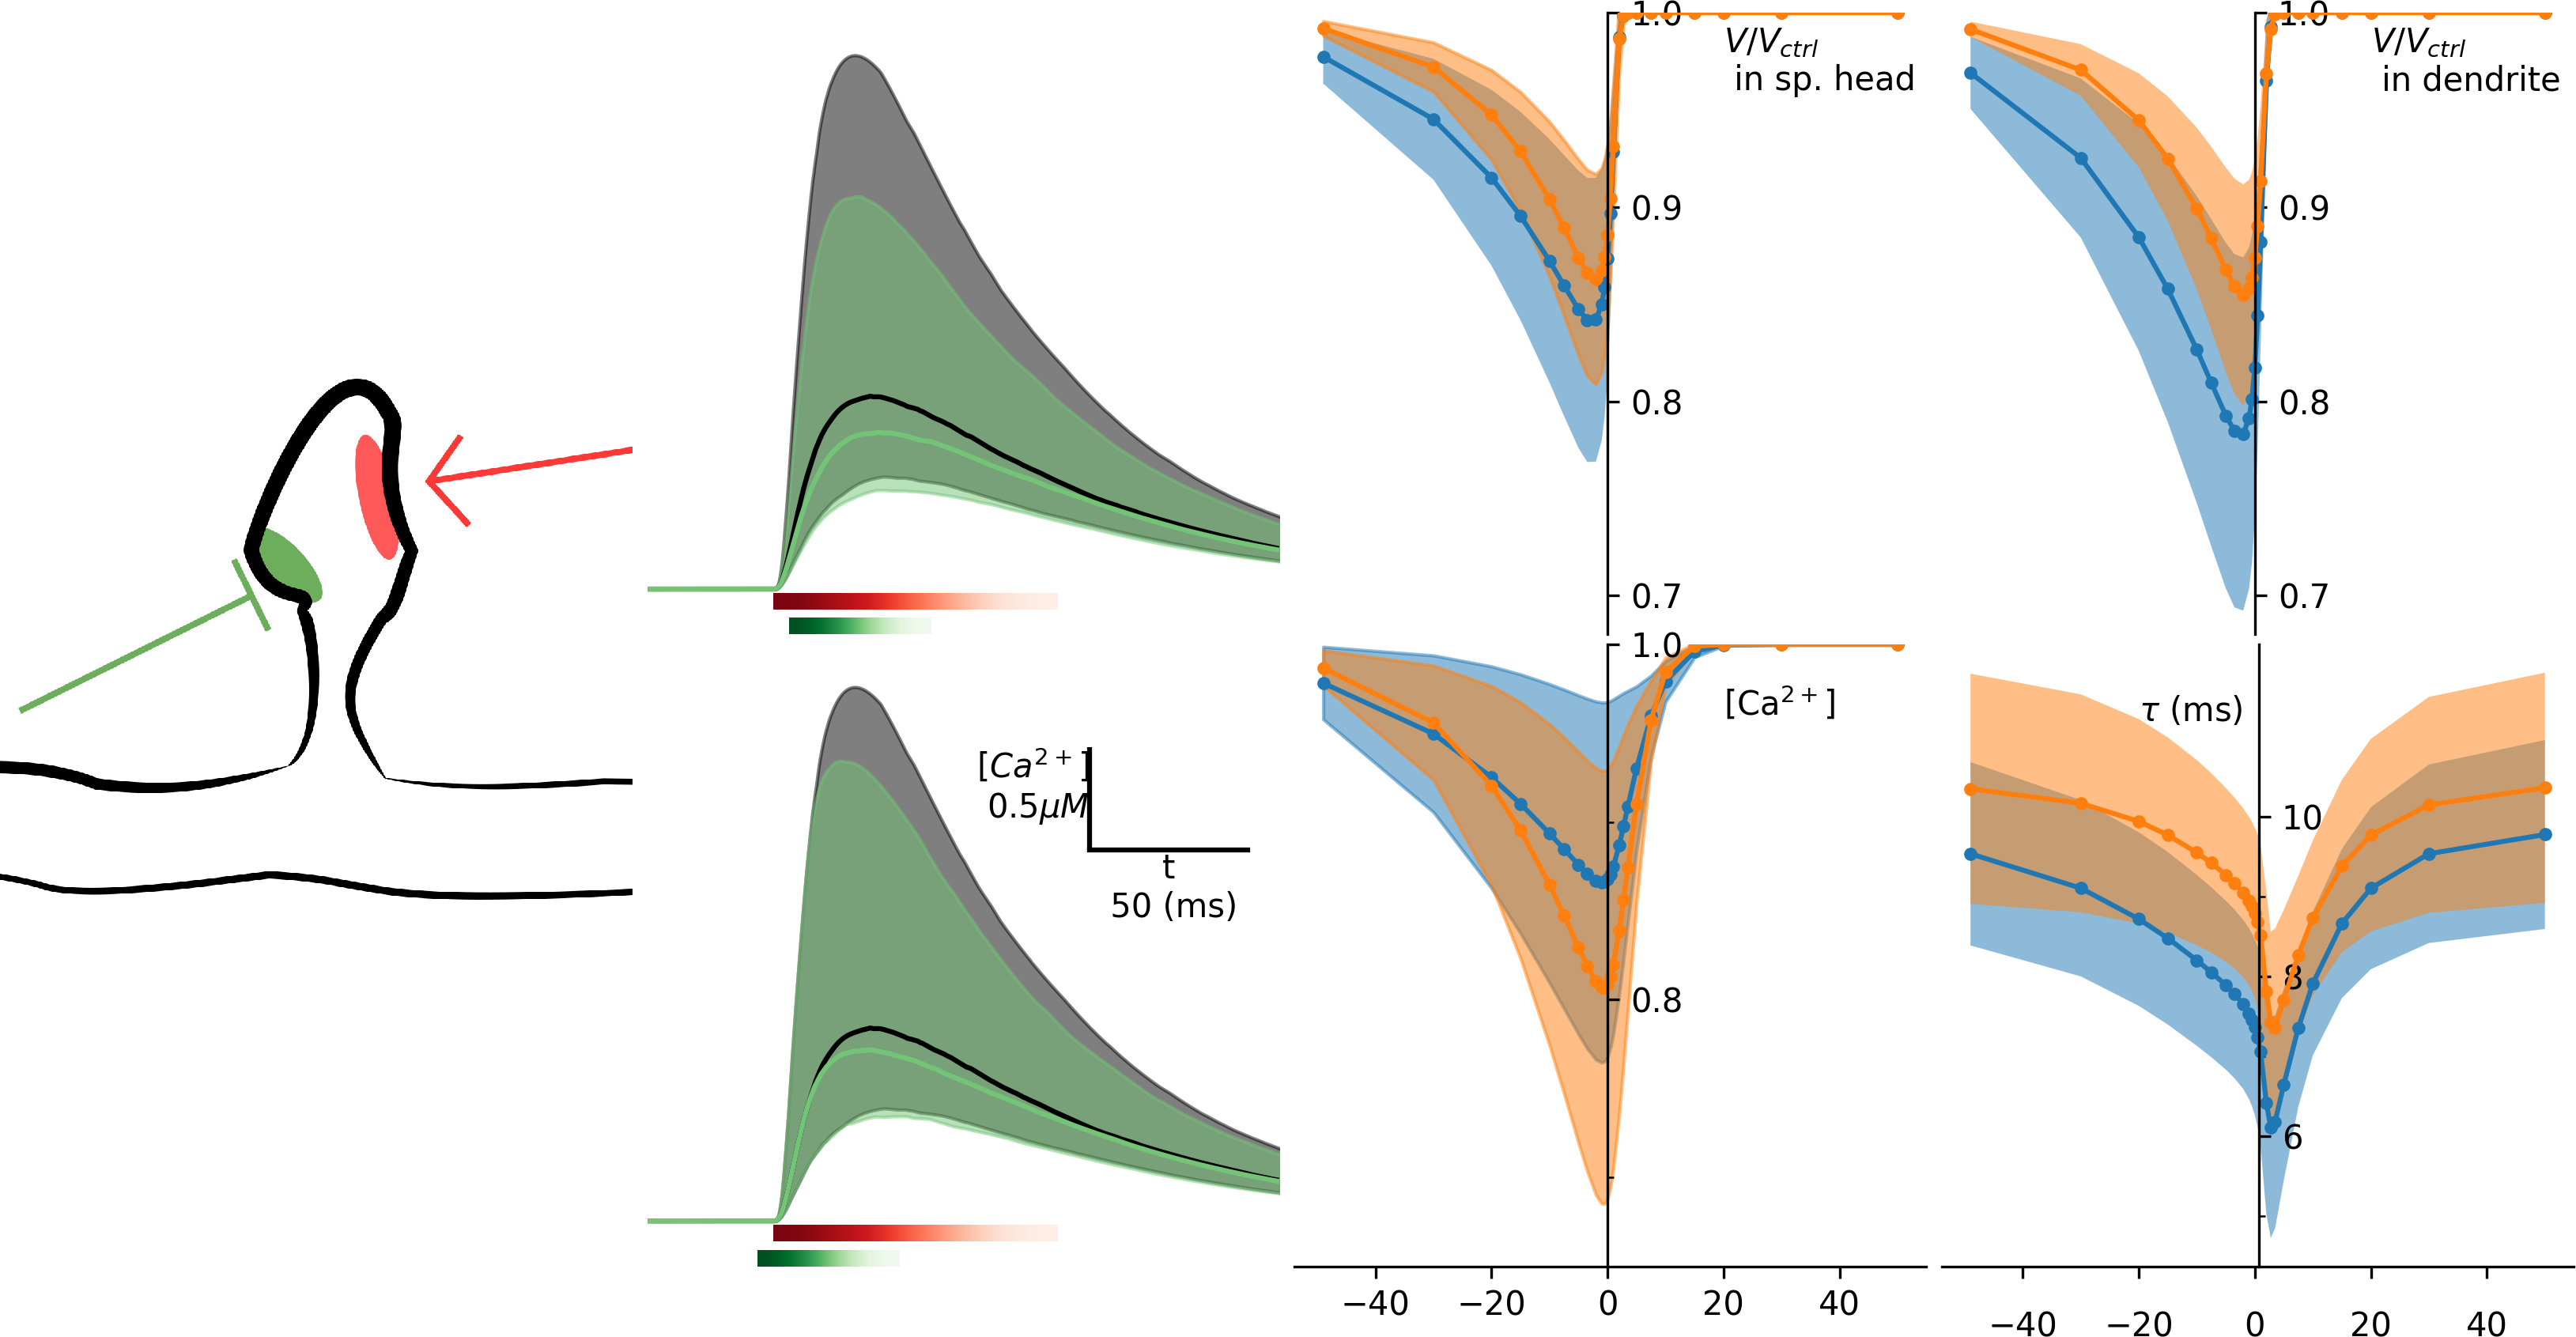
\includegraphics[width=1.0\linewidth]{f2}
\caption{{\bf Timing of inhibition.} 
Panel a show a sketch of the protocol for the timing of inhibition. In case  I (black) a glutamate release is simulated at a (bs) DiS spine and after $\Delta t$, GABA release is simulated and inhibitory synapse is activated. In case II (violet) GABA is released first and after $-\Delta t$ time  glutamate is simulated. The effect on the depolarization in the spine head is shown in panel b1 when $\Delta t= 15$ ms. Note that inhibition effect is shunting the membrane, so when it arrives first its effect is not apparent until glutamate arrives. In panel b2, the effect on the intracellular Calcium is shown.
In panel c1 and c3, we show the the amplitude of the depolarization and calcium concentration as a function of $\Delta t$ (negative values: GABA arrives first; positive values: glutamate arrives first), normalized to the case without inhibition. In panel c2, we show the decaying time of the depolarization as a function of $\Delta t$.
%In right panel, we show its dependence on a correlated Poisson train, as a function of (THE VARIABLE critical for this).
}\label{fig:TimingInhibition}
\end{figure}

One of the main effects of inhibition in the dendrite is to locally shunt the membrane when incoming EPSPs arrive (refs). 
%We include inhibitory synaptic inputs in the model blocks corresponding to spines and dendritic shafts. 
This depends on the chloride reversal potential and resting potential of the cell. Although it changes during development and other conditions, we will consider here both at -70 mV. If inihibition and excitation are uncorrelated, the former only have an average effect reducing EPSPs. However correlated inhibition may have a much stronger effect. To test this, we include a inhibitory contact in the compartment of the spine head, panel a in Fig.\ref{fig:TimingInhibition}. 
%\def\Cl{\text{Cl}}
%\begin{equation}
%E_{\Cl^-} = -\frac{RT}{F} \text{log}\frac{[\Cl^-]_o}{[\Cl^+]_i}
%\end{equation}


%The overall effect can be estimated (and measured!) in the soma, however the model provides a way to see its effect in the spine head or in the dendritic branch with the implication this has. 
In panels b1 and b2 we show the effect of inhibition in the intracellular Calcium in the spine head. It features the distribution of Calcium transients due to an EPSP without inhibition in black, and in green when inhibition arrives 5 ms after (panel b1) or 5 ms before the EPSP (panel b2). The activation of the excitatory event is marked in red  below the curves, while the inhibitory one is in green.

To study the effects for signal integration, we extract the amplitude of the Calcium and Voltage transients. In order to see the effect of inhibition, we normalise the amplitude to a case with no inhibition. In panel c, we show the  in the spine head both for voltage (blue) and Calcium (orange), and for DiS (dark colors) and SiS with an inhibitory synapse nearby (lighter colors). When inhibition comes first, the GABAergic current has the chance of shunting the depolarization peak. In contrast, when it comes \underline{last} (?) the effect on the amplitude disappears (except for a very small window of time). The asymmetry is manifest, but exhibits slower dynamics in Calcium compared to voltage. This is due to the slower dynamics of NMDAR-mediated currents, which account for most of  Calcium entry in spine heads. The effect of inhibition inside the spine is clearly \textbf{(???)} different in DiS (dark colors) as compared to SiS (lighter colors). 

The effect of the interplay of a single inhibitory and single excitatory input in the soma and in dendritic shaft are shown in panel f of Fig.~\ref{fig:TimingInhibition}. Similarly to the spine head (in panel e), the asymmetry appears for the depolarization as a functon of the delay of inhibition. However, there is no big(??) difference of the effect of inhibition depending on its location: in spine (dark blue) in the shaft closer to the soma (light green) or further from the soma   (light purple) (there may be difference with this case - check). 


\subsubsection*{Dendritic integration - synaptic gating}
\paragraph*{Attenuation of the signal.} Signal as a function of the distance. Electrotonic concept (Rall). Chirality broken (REFs?). Determination of the electrotonic length. Shunting Levels with inhibition along the dendrite: What happens with inhibition: in spine/ out of spine/ 
in dendritic branch (REF: paper journal club).



\begin{figure}[htb!]
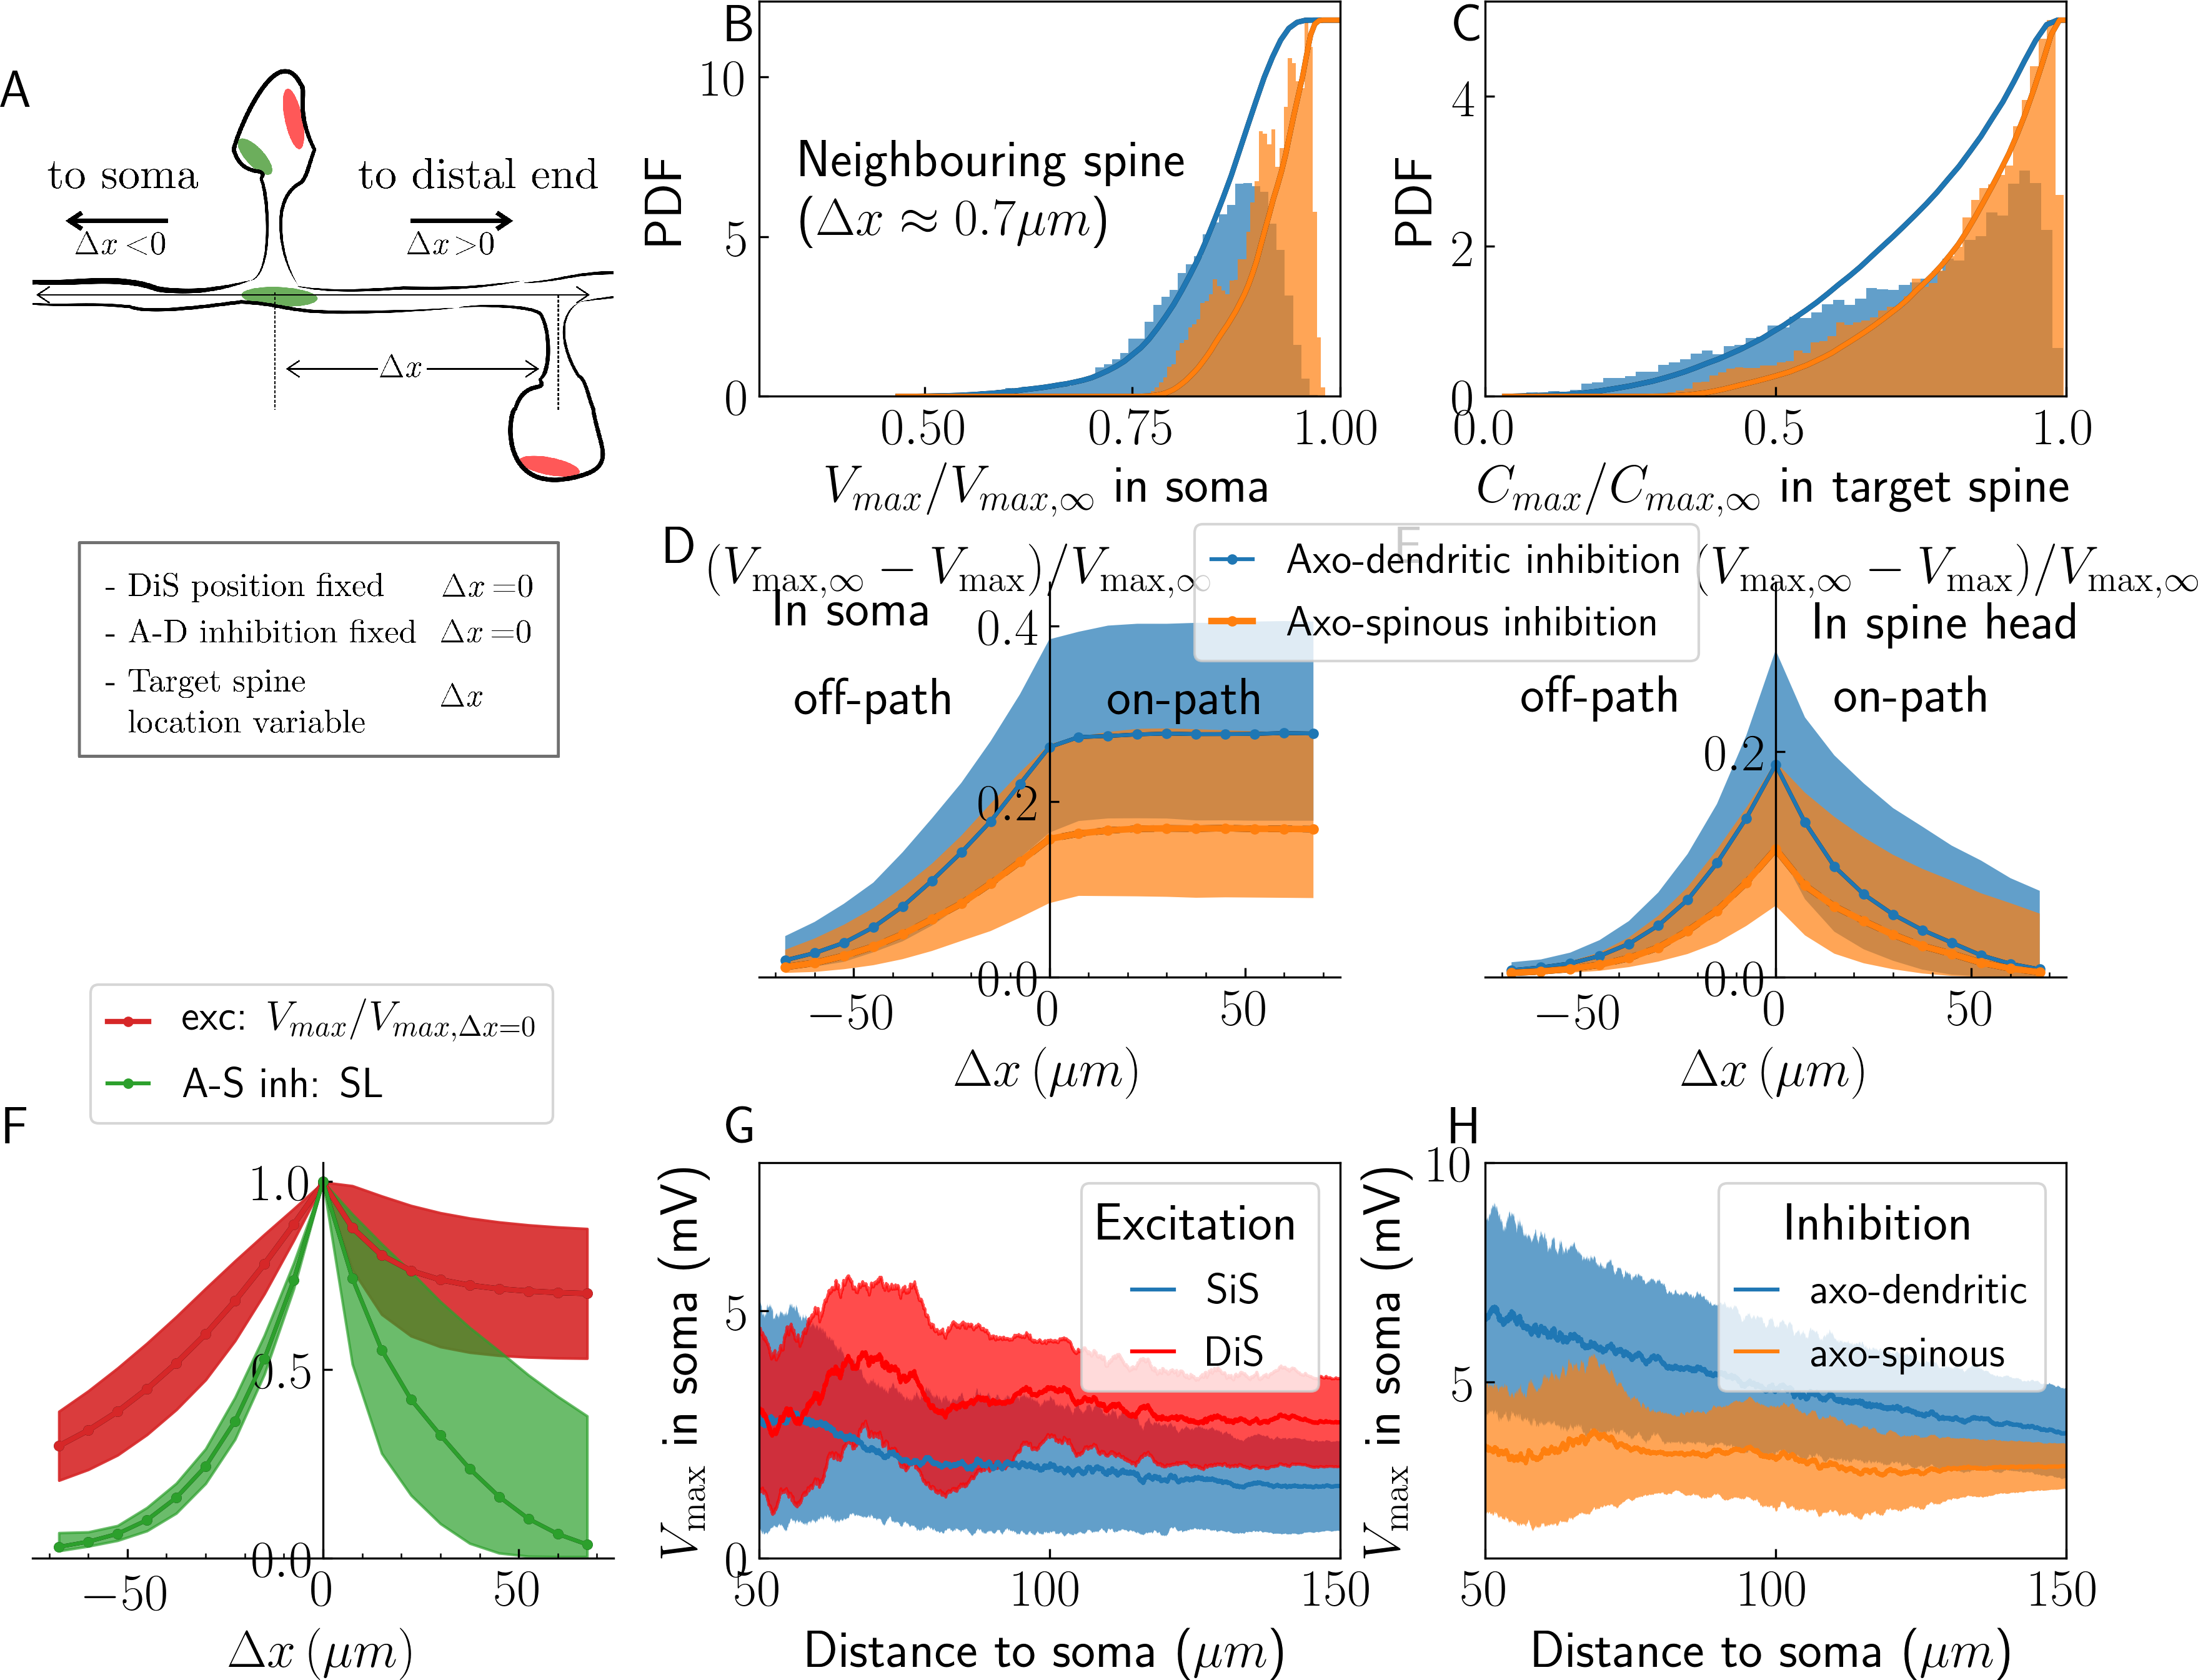
\includegraphics[width=1.0\linewidth]{f3}
\caption{{\bf Dendritic integration.}   Panel a -- sketch spines distance and interaction. Panel f -- attenuation of the signal as a function of the distance to the synapse for both excitatory (red) and inhibitory synapses (green) in DiS. 
%In right panel, we show its dependence on a correlated Poisson train, as a function of (THE VARIABLE critical for this).
}\label{fig:Dendritic integratio}
\end{figure}


On this aspect of dendritic integration we can study how the effect depends on the distance to the synapse for both excitatory and inhibitory synapse. For the excitatory synapse is relatively straightforward, we compare the amplitude of the EPSP along the dendrite with the value in front of the spine. For the inhibitory synapse instead, the effect is usually shunting the membrane. For those cases when there is a hyperpolarization or a depolarization due to inhibition, the effect is rather small, and what would happen there -- similar to excitation?? To define the effect of shunting we place the second spine at a distance x of the axo-spinal contact and elicite there an EPSP, with an amplitude  wihout inhibition $V_0$. Now, we repeat the same experiment with axo-spinal inhibition arriving $5$ ms before the EPSP(what happens if it is later? Nothing?). The decrease in amplitude of the latter, $V_{i}(x)<V_0$, is the shunting effect due to the inhibitory synapse. To quantify it we consider the diference of the two amplitudes normalized to $V_0$. In panel d, we show the ratio of this quantity compared to having the spine next to the axo-spinal inhibitory contact
\[ SL(x) = \frac{V_0-V_i(x)}{V_0-V_i(0)}
\]


\paragraph*{Gating synapse.} An interesting phenomenon already described in the literature is synaptic gating (Ref). This refers to the fact that some inhibitory inputs may selectively gate excitatory inputs decreasing their amplitude. Inhibitory synapses in DiS might be an ideal candidate to drive it. We design a different protocol to address this problem, we consider two spines in a small piece of dendrite in the dendritic arbor we simulate. One of the spines is dually-innervated (the other is extrated from the whole set of spines). We simulate an EPSP incoming in the second spine and measure its effect in the soma or in the dendrite. This will be the control experiment. Then, we repeat it and have inhibition activated slightly before the EPSP in the DiS ($\Delta t =-5\,ms$). We show the histogram of the normalised depolarization amplitudes in the soma in panel b (very similar to the one observed in the dendrite). Similarly, we repeat this protocol, but activating an inhibitory synapse in the dendritic shaft instead of the one in the DiS. The distribution is shown in red. There is a clear shift, ~??$\%$ vs ??$\%$. Note that the fact that axo-dendritic synapses are larger than axo-spinal ones makes this difference stronger. In the case of similar sizes, the difference in the two effects is roughly ??$\%$ (appendix). The effect can be seen in the intracellular Calcium concentration in the spine head of the second spine, panel c. ({\bf Is the difference in the median of the distribution the fact that we are sampling all the spines?}). The shift in the median from axo-dendritic to axo-spinal inhibition is ??$\%$. {\bf Should we speak about literature inhibition and Calcium - Journal club}.


%The same effect can be shown case by case by taking the difference in amplitudes and normalising. The distribution is shown in panel f (orange). The median for this is roughly 10\% and the probability that the effect is equal or smaller in the shaft than in the spine is 0.2. However this comparison takes into account all the variability of synapses, if instead we take same synaptic size for both axo-dendritic and axo-spinal inhibition, the distribution (blue) is shifted and becomes narrower. The probability of having smaller transients due to inhibition in shaft is smaller than 0.003. When looking at intracellular Calcium there is a similar situation. If they were to have the same area, the effect of shaft inhibition would be 15\% stronger (appendix -figure red/blue).


\subsection*{STDP}

\begin{figure}[htb!]
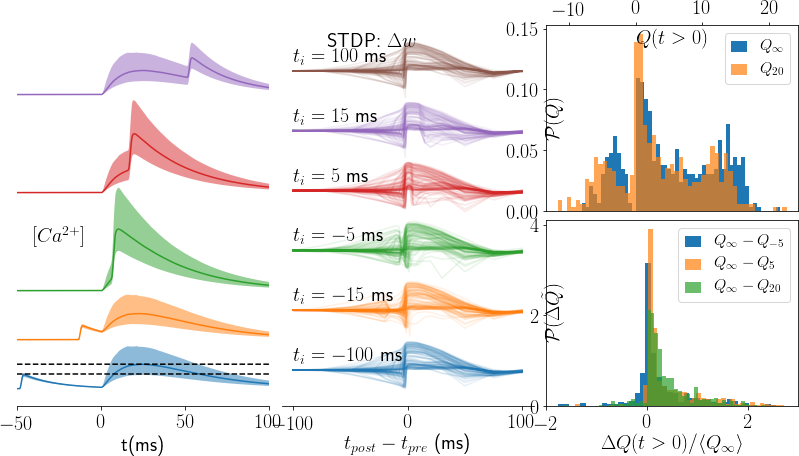
\includegraphics[width=1.0\linewidth]{f4}
\caption{{\bf STDPs.} Panel a shows Calcium transients for a STDP protocol for several cases of $\Delta t_1$, timing between (excitatory) pre- and postsynaptic AP. Panel b shows the heterogeneity of STDPs curves we obtain in a protocol ofo 100x 0.5 Hz. In panel c, colormap of 2 $\theta$ with probability of finding DPD curves. Panel d shows how inhibition changes STDPs curves for those typical DPD' curves found in SSx. 
}\label{fig:stdps}
\end{figure}



\subsection*{Active conductances}\label{sec:active conductances}

This section includes modeling bAPs to model Hebbian STDP in DiS. Varying the timing between E/I stimuli (let alone the respective synaptic strengths, responsiveness and channel kinetics) will give insights on the fine regulation of Hebbian STDP by axo-spinal inhibitory synapses.

\section*{Discussion / Conclusion}

%\nolinenumbers

% Either type in your references using
% \begin{thebibliography}{}
% \bibitem{}
% Text
% \end{thebibliography}
%
% or
%
% Compile your BiBTeX database using our plos2015.bst
% style file and paste the contents of your .bbl file
% here. See http://journals.plos.org/plosone/s/latex for 
% step-by-step instructions.
% 


\section*{Materials and methods}
\subsection*{Animals}
All animals were handled according to protocols approved by French authorities. Timed-pregnant female mice were maintained in a 12 hr light/ dark cycle and obtained by overnight breeding with males of the same strain. For timed-pregnant mating, noon after mating is considered E0.5. Adults correspond to mice between P84 and P129.

\subsection*{In utero cortical electroporation}
In   utero cortical   electroporation   was   performed at   E15.5 on   timed   pregnant RjOrl:SWISS females (Janvier Labs) for electrophysiology or C57BL/6Jfemales Janvier Labs in Figure 5. 
The previously described protocol for in utero cortical  electroporation (Hand  and  Polleux,  2011)was  modified  as  follows.  We  used  timed  pregnant  RjOrl:SWISS females. Endotoxin-free  DNA  was injected  using  a  glass  pipette  into  one  ventricle  of  the  mouse  embryos.  The  volume  of  injected  DNA  was  adjusted depending  on  the  experiments.  Electroporation  was  performed  at  E15.5  using  a  square  wave  electroporator  (ECM 830,  BTX)  and  gold  paddles.  The  electroporation  settings  were:  4  pulses  of  40  V  for  50  ms  with  500  ms  interval. 

\subsection*{Tissue preparation}

\appendix
\section{Methods}

\section{Bootstrap}
The statistics of the set of measurements we have presented in this manuscript is non-trivial. We do not only refer to the appearance of log-normal like distributions, with not-so heavier tails, but also the existence of non-linear correlations between observables. Although some correlations can be modeled in a relative simple way, e.g., area vs volume of the spine head (REF? Yuste), in other cases it requires a bigger effort, e.g., {\bf the figure with weird correlation 1/length: length vs volume or something like that (REF)}. Also, we are not interested in the effect of this particular snapshot of spines, but rather in the effect of generic spines that we have had access to, through the snapshot that we took. We use (smooth) bootstrap methods to re-sample the distribution with the correlations. We use the synthetically generated spines (that have similar statistical properties to those we physically measured) to sample the distribution of electrochemical effects in a neuron model environment.

{\bf Bootstrap.} Bootstrap methods consist in re-sampling measured data in a random fashion. Our set of data consist in a matrix $\mathcal{D}$ of dimension $NxN_O$, with $N=370$ number of spines and $N_O = 25$ number of observables. Note that some of the observables may not be used in the {\bf simulations}. If we consider measurements of each spine completely independent, a simple bootstrapping technique to generate a new set $\mathcal{D}'$ of $M$ spines consists in selecting them randomly (with possible repetition) from the rows of $\mathcal{D}$. However, if we want to sample better the distribution of effects, we want to smear the distributions of parameters retaining its features. Even if there is correlation between variables, we will assume that the noise in each variable is small and independent from each other. To estimate the amount of noise we can introduce, let us study it in a particular example: the length of the neck. 


\def\L{\mathcal{L}}
We calculate first the (cumulative) distribution of the original set of length of spine necks $\L = \{l_i, i=1,\ldots,370\}$, comprising 370 cases, Fig.~\ref{fig:FFT score dist}. We bootstrap the data set by producing $M=500$ random indices from 0 to 370 (with repetition) and generating a new synthetic set $\L' =  \{l'_{j_1},\ldots, l'_{j_{500}}\, /\, l_j' = l_j (1+\sigma\xi) \}$ where $\xi$ is a random gaussian variable with variance 1 and $\sigma$ the noise level. We calculate the distribution for $\L'$ and perform a 2 sample Kolmogorov-Smirnov test, obtaining a $p$--value. We repeat this procedure 1000 times for each studied noise level and obtain statistics.In Fig.~\ref{fig:FFT score dist}, we show for different noise levels the fraction of synthetic sets whose $p$--value is below various thresholds (color coded). Since we want to keep small noise levels as well, a noise level of $\sigma=0.1$ seems to avoid generating synthetic sets with $p$--value below 0.05, a lax constraint (to consider them different).  
\begin{figure}[htb!]
    \centering
    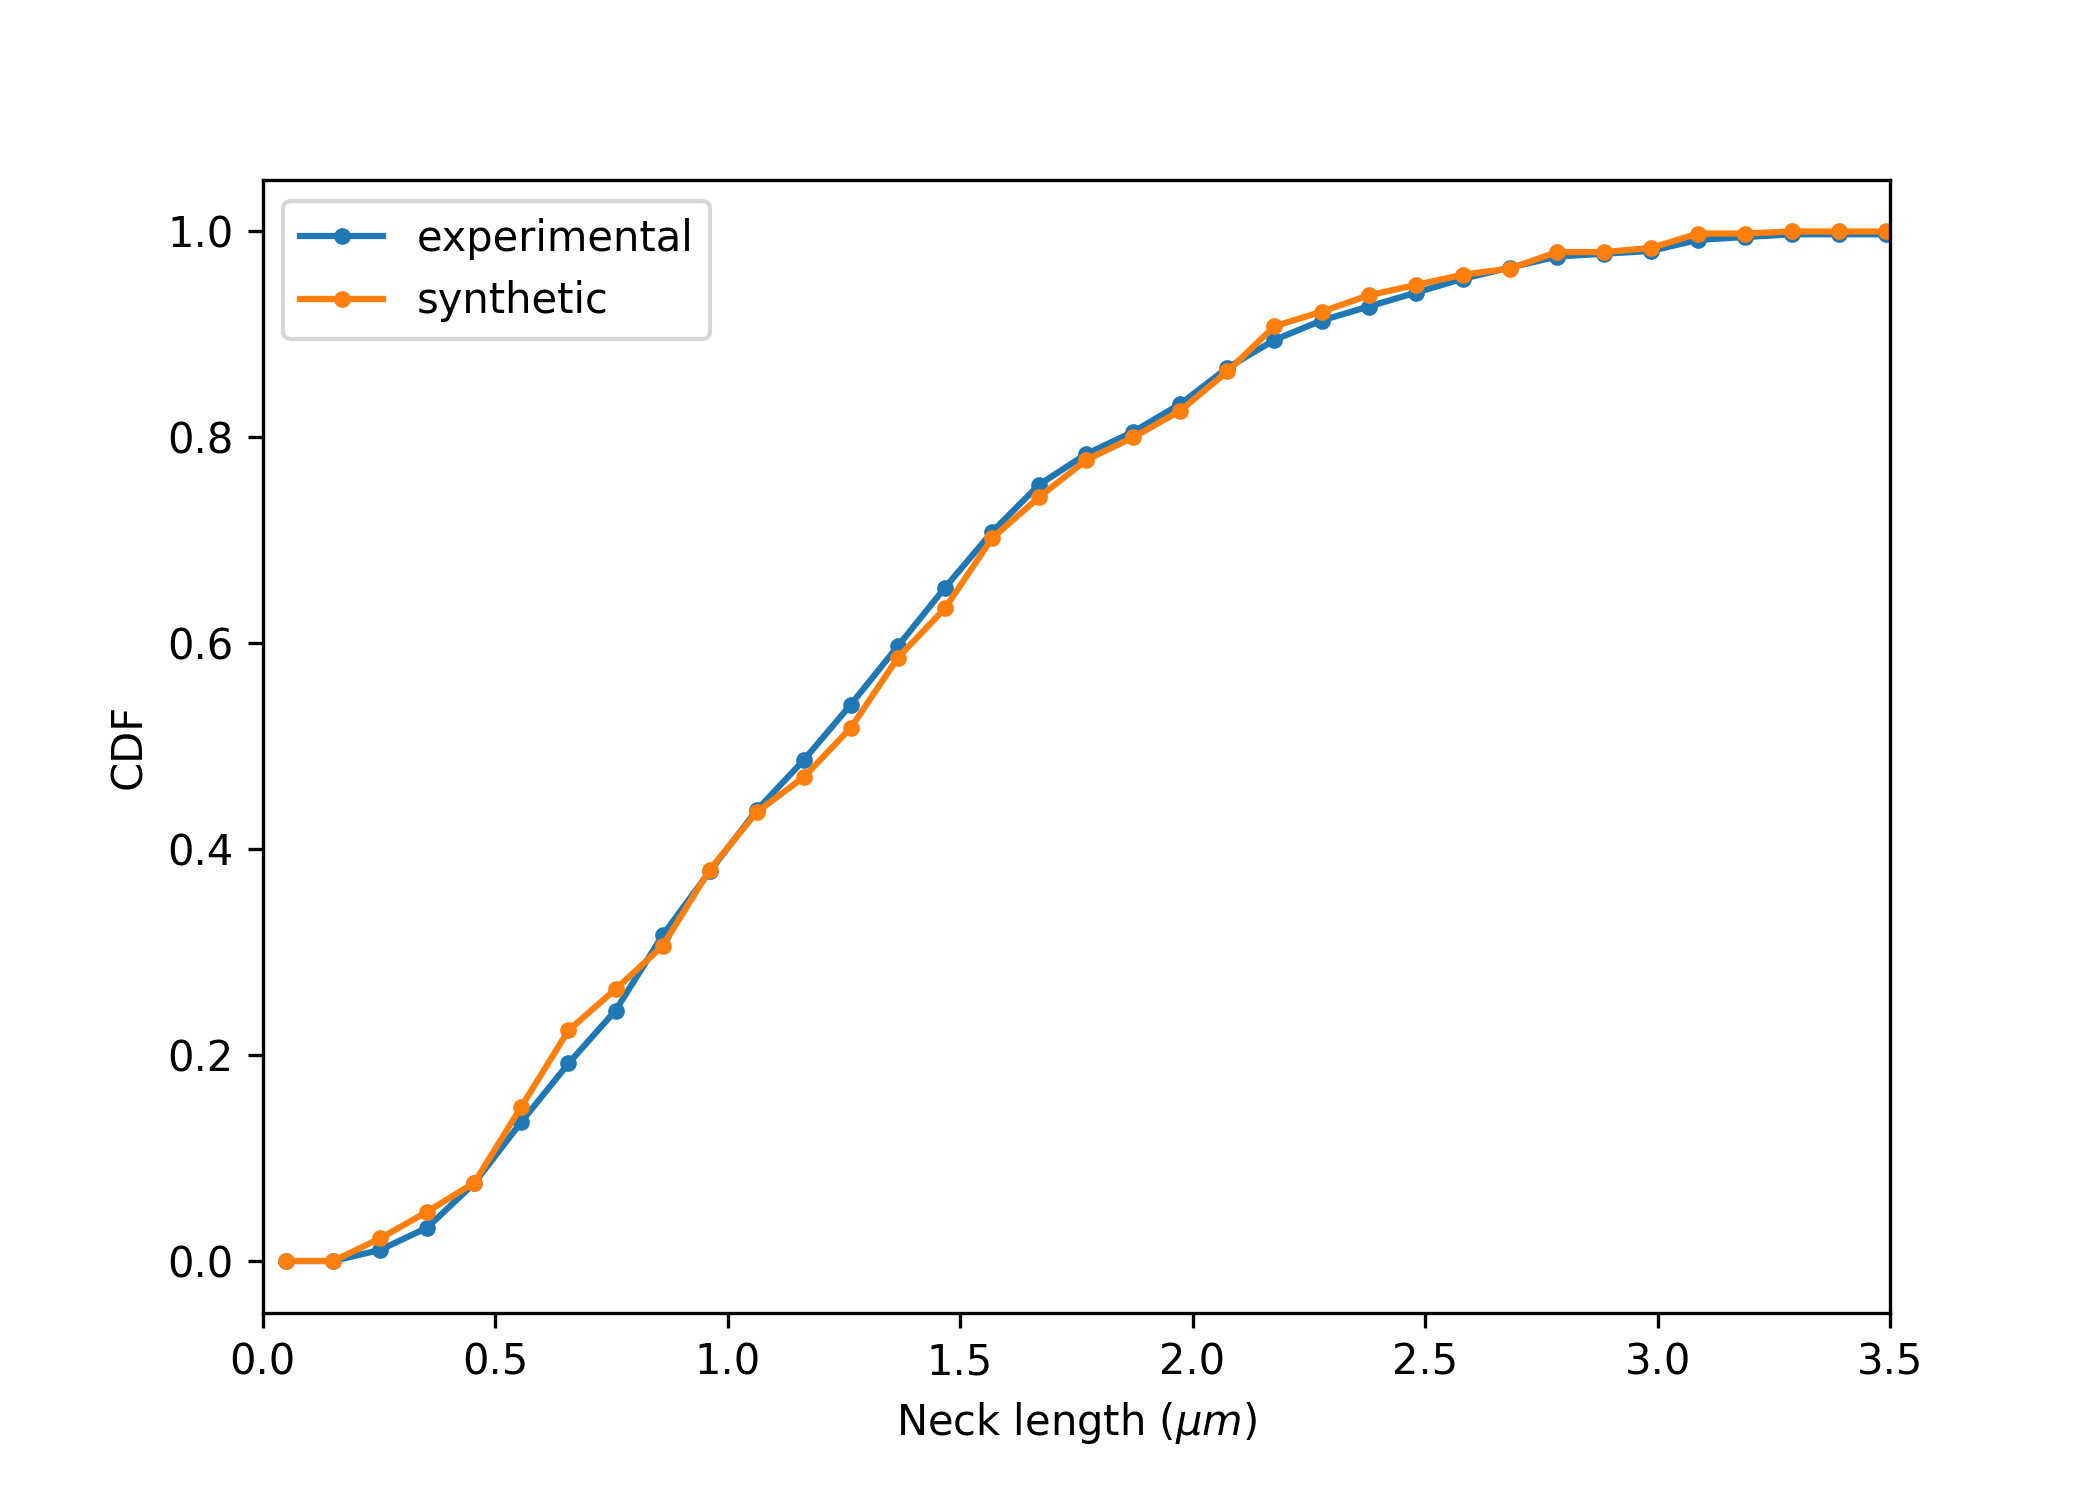
\includegraphics[width=0.48\linewidth]{cdfLnBootstrap}
    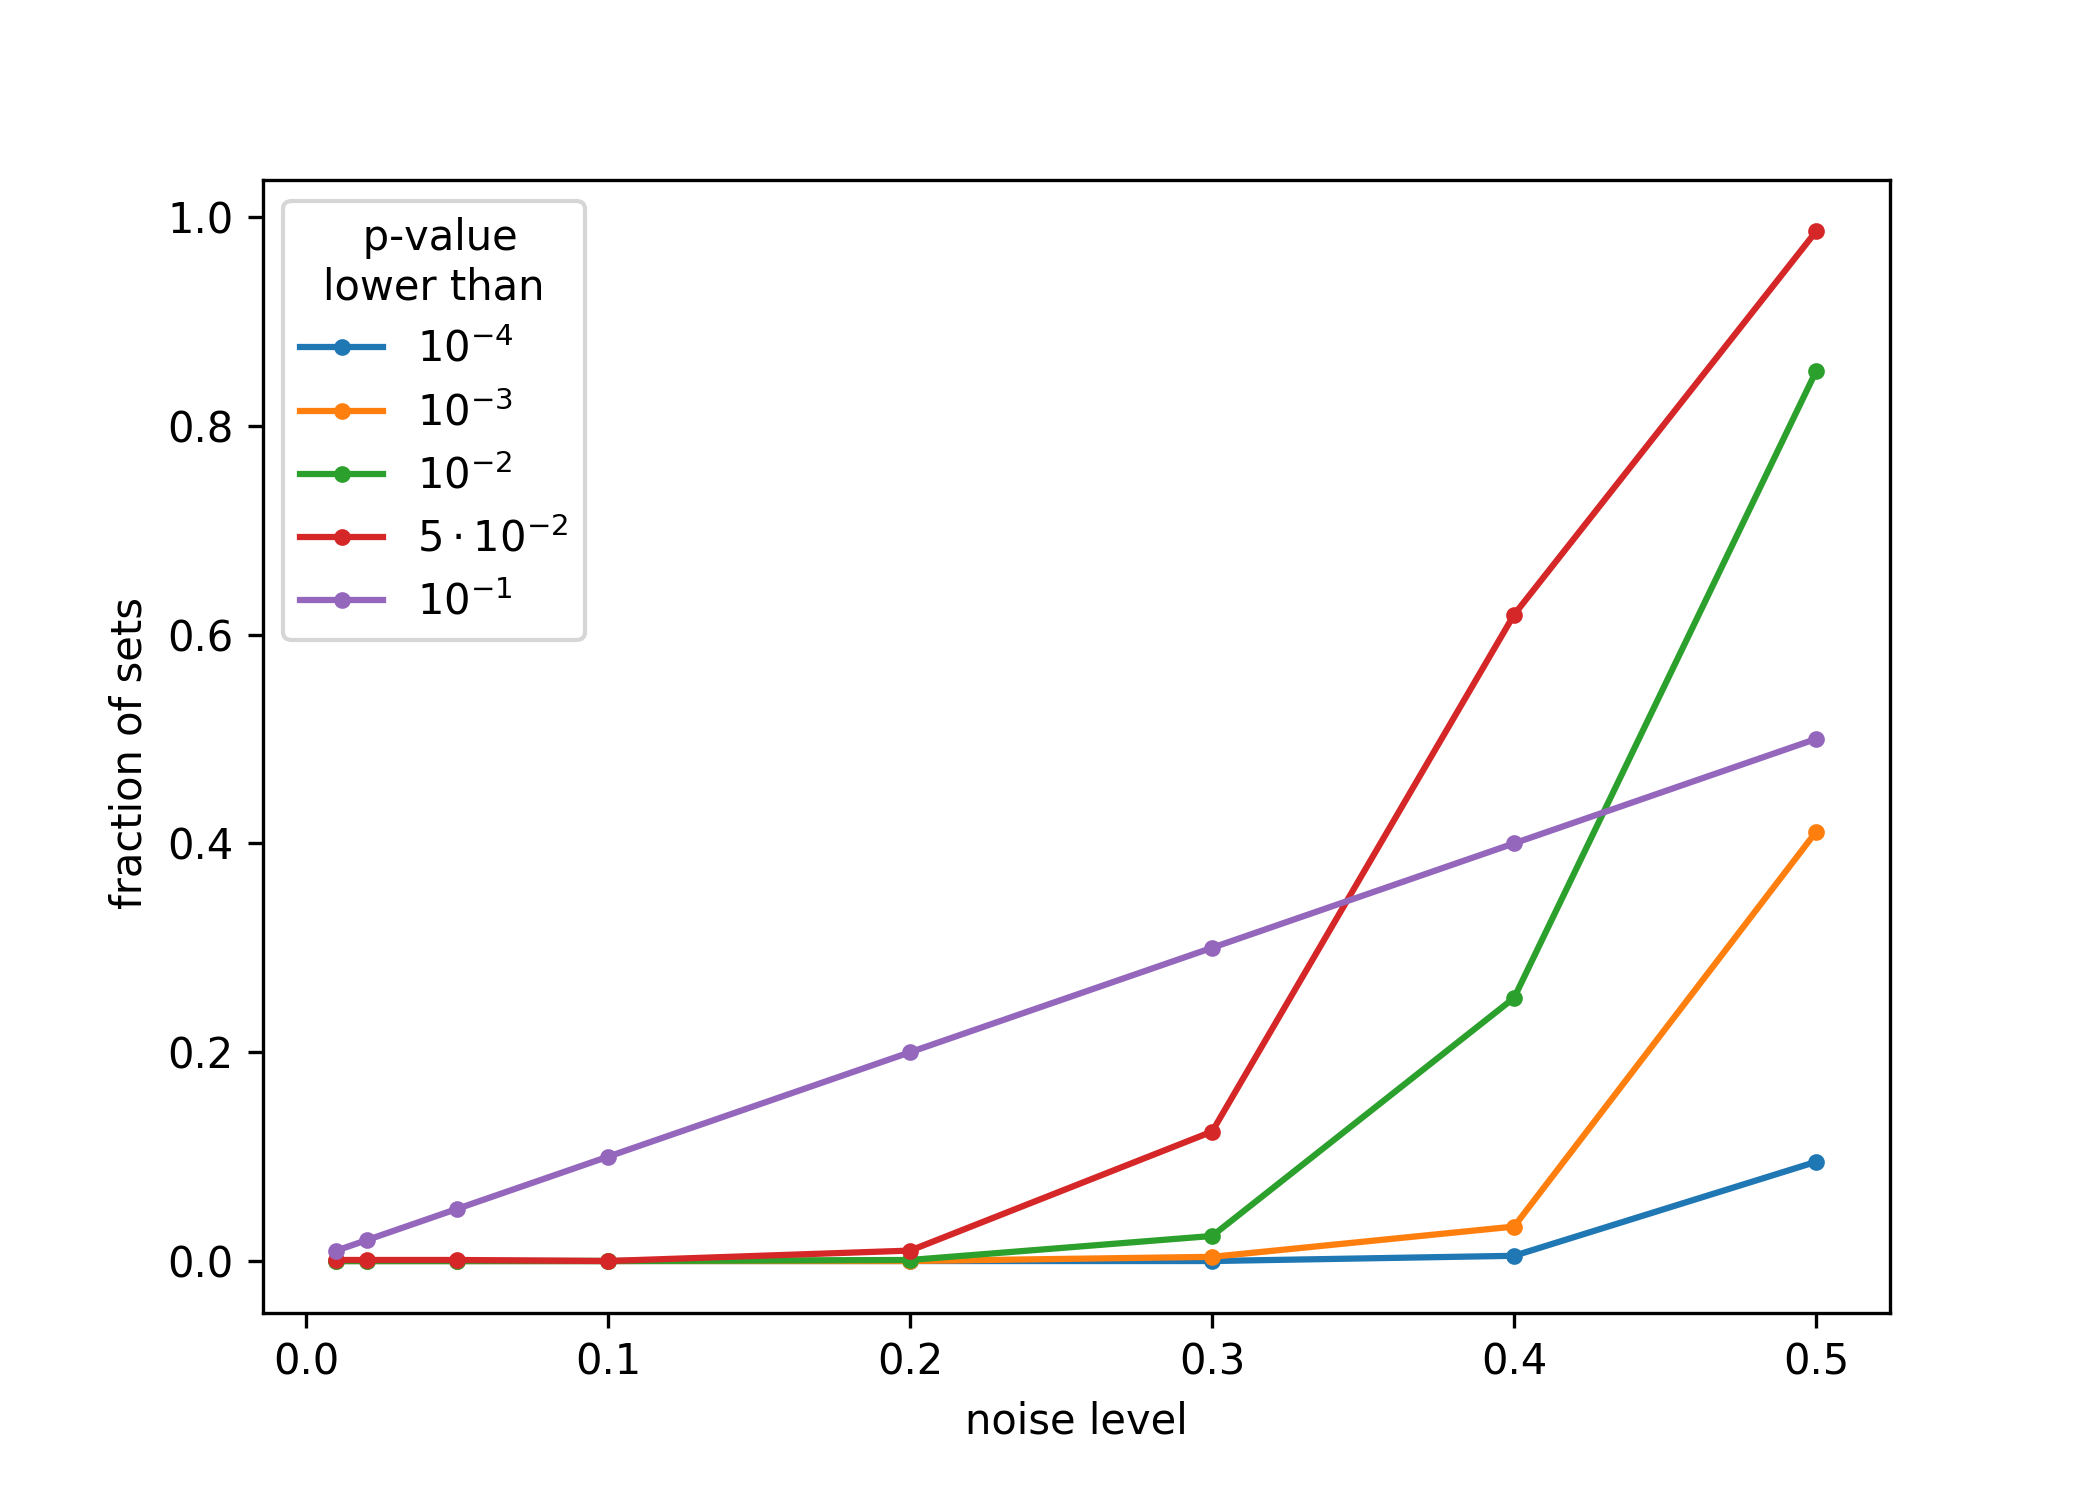
\includegraphics[width=0.48\linewidth]{fraction_noiselevel_Ln}
    \caption{Panel a shows cumulative distribution of the experimental length of the spine necks compared to a synthetic set with noise level 0. 2 sample KS test gives a p-value of 0.95. Panel b shows fraction of spine sets whose neck length distribution produces a p-value lower than various thresholds, in a 2 sample KS test with the experimental distribution as a reference. This is shown as a function of the amount of gaussian noise introduced in smoothed kernel for bootstrap.}
%Ornstein-Uhlenbeck processes 
    \label{fig:FFT score dist}
\end{figure}

We have checked that $\sigma=0.1$ is a correct noise level for other quantities subjected to noise in their measurements. New synthetic spines are produced by choosing one index from 0 to $N$ and introducing noise as gaussian random variables in each one of the selected variables (independently). Note that we do not select independently different features, by selecting $N_O=25$ random indices, with the aim of keeping the correlations associated to the system we have had access.

{\bf Paragraph about the boons of bootstrapping!}. DiS are very few, we now have many to play with. It can be used to test other stuff. What else? It gives an estimate of errors of the measurements as well. Anything else?


\begin{thebibliography}{10}

%\bibitem{bib1}
%Conant GC, Wolfe KH.
%\newblock {{T}urning a hobby into a job: how duplicated genes find new
%  functions}.
%\newblock Nat Rev Genet. 2008 Dec;9(12):938--950.

\end{thebibliography}



\end{document}

